To better understand the scenario of machine learning studies in medicine in recent years, and specifically in the field of mental health, a systematic literature review (SLR) was brought to analysis.
~\citet{Burke2019} focused its attention on suicide-related applications and employed a methodology oriented by inclusion and exclusion criteria, where papers from multiple sources were processed through a systematic pipeline.

The SLR targeted papers published until February 2018 in the PsycINFO, PsycARTICLES, ERIC, CINAHL and MEDLIN databases.
From an initial set of 288 retrieved studies, derived by search terms of methodological (e.g.\ "machine learning", "data mining" and "big data") and domain ("suicide", "self-injury", "suicide ideation") imprint, only 35 papers met the inclusion criteria and went on to further analysis.

As for the conclusions of the review, we are interested mainly in its insights on the successes and difficulties of previously employed ML algorithms in problems with similar characteristics to ours - to predict suicide ideation.
The study was able to demonstrate the potential of ML algorithms in the mental health field;
it was shown that this branch of technology can greatly improve the prediction performance of mental disorders.
Furthermore, the exploration and finding of predictor variables replicate established results but also find novel variables and identifies subgroups of interest.
This SLR also emphasizes the importance of the interpretability of the models and their trade-off over performance.
To that extent, this subset of the literature tends to favor simpler predictors like decision trees.
As \autoref{fig:burke-algorithm-prevalence} shows, over 60\% of the analysed papers employed DTs, while ANNs (a generally less interpretable model, though a strong performer in a myriad of applications) appeared only in about 10\% of the articles.

\citet{Burke2019} separate the study of suicide into distinct (though sometimes intersecting) categories: suicide death, suicide attempt, suicide planning, and suicide ideation.
SI studies (a small subset of only 10 papers in this SLR) used both cross-sectional and longitudinal designs (with one to five years follow-ups), considering data from population samples distinct in age, locale, and mental health.
The trained models incorporated, on average, 32 attributes (ranging from 3 to 62), and each study used one to four (M=1.6) ML methods.
Almost all of the ten papers used structure data, safe from one that employed an NLP approach.
As for the performance metrics, however, the inconsistency in strict and standardized reporting is evident.
Some papers do not show any performance estimation whatsoever, while others generally do not share the same indicators and scores (reporting exclusively AUC-ROC, accuracy, or sensitivity and specificity, etc.).
Along with the small paper sample size, this makes the effort to derive statistics on their models' performance futile.

Nevertheless, the reported metrics are indicative of the potential of employing the algorithms from \autoref{fig:burke-algorithm-prevalence} in the prediction of suicide ideation.
As~\citet{Burke2019} compiled, suicide ideation prediction studies reported AUC values ranging from 0.8 with DTs~\cite{Handley2014} to 0.92 with DTs and RFs~\cite{Gradus2017}, and sensitivity and specificity reaching 0.88 and 0.94~\cite{Just2017} with decision trees, neural networks and Support Vector Machines (SVMs), although considering only 34 data points, half of which were of the positive class).

Besides the gaps and inconsistencies in reported performance, Burke's SLR brings to light the lack of consistency and depth in treatment and discussions of class imbalance in training data in the analysed studies.
While many papers report AUC, which better describes the performance than just the accuracy, it still falls short in completely describing the actual performance of the predictor in the presence of class imbalance~\cite{Burke2019}.
And while some papers report precision and recall, few studies address the problem of unbalanced data in their sampling and training.

\begin{figure}[h]
    \caption{Algorithms prevalence from~\citet{Burke2019}}
    \centerline{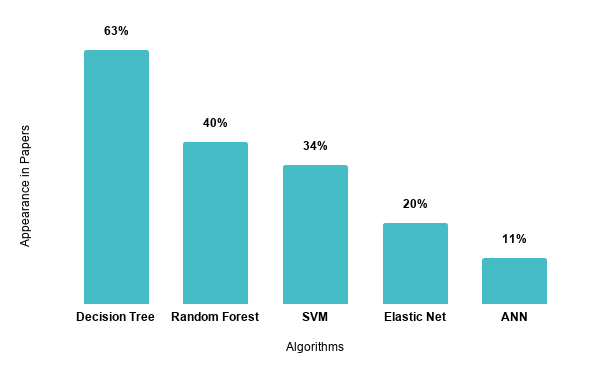
\includegraphics[scale=.75]{fig_burke_alg_usage.png}}
    \label{fig:burke-algorithm-prevalence}
    \legend{Source: Author}
\end{figure}

That said, even though the beneficial attribute selection (for data dimensionality reduction) and class-imbalance mitigation techniques are oftentimes lacking in classifications problems in the context of mental health ~\cite{Burke2019}, that is not always the case.
An example of successful attribute selection is presented in ~\cite{Barros2017}, which used a wrapper-based method in a Chilean mental-health patients dataset to reduce the feature set size from 343 to 22, reporting sensibility and specificity between 0.7 and 0.8, approximately.
On the other hand, in the context of class-imbalance reduction, ~\citet{Schubach2017}} employs both downsampling of the negative class and oversampling of the positive class (with the SMOTE algorithm) to balance data partitions and train a random forest on each, afterward combining them in what is described as an ensemble of ensembles.
The models' performance estimation from~\citet{Schubach2017} varied substantially depending on the evaluated dataset, achieving at best around 0.7 area under a precision and recall curve, but at worst barely over 0.4.
That said, the calculated AUCROC was always around 0.98 (again showing a problem in relying only on this metric).

Since the afore-mentioned SLR did not review works after February 2018~\cite{Burke2019}, it is also worth mentioning some related works developed since then - again, searching for insights on their achievements and limitations, bringing to light their similarities to our study.

With a similar problem to the one our work aims to solve, future risk of suicidal thoughts was chosen as the outcome variable to the models of ~\citet{Roy2020}, although the employed data was unstructured (text, from Tweeter).
The study considered a vast amount of tweets per individual, but on the other hand, the suicide ideation cases in the dataset were less than 300.
That said, the study achieved a high AUCROC value of 0.88 using a model that combines the outputs of several neural networks using a random forest.

Using structured data from Korean population samples, two studies~\cite{Oh2020, Jung2019} also tackled problems akin to ours, with similar approaches too.
Both proposed to solve the problem of classification of suicide ideation (with our without suicide attempt), but with different datasets.
The first focused adults~\cite{Oh2020} and the second on adolescents~\cite{Jung2019}.
With over 16,400 instances, the Korea National Health and Nutritional Examination Survey (KNHNES) data employed in~\citet{Oh2020} is more than four times larger in this regard than our restricted (to common mental disorders) sample of the ELSA-Brasil dataset.
On the other hand, although the Korean Young Risk Behavior Web-basedSurvey (KYRBWS) dataset from~\citet{Jung2019} included data from over 62,200 adolescents, ~\citet{Jung2019} employed a drastic downsampling strategy in its preprocessing, achieving class balance to the cost of reducing the instances count to approximately 15,300 - just as the data in ~\citet{Oh2020}, amounting to approximately 400\% of our dataset size.

As far as assessed variables are concerned, a key difference between a fully automatic approach to variable selection (as we propose in Chapter~\ref{ch:methodology}) and the one from~\citet{Oh2020} is that the study resorted to filtering based on the manual inspection and review of two health professionals, reducing the dimensionality from 800 variables to only 48.
That said, ~\citet{Oh2020} also employed wrapper-based feature selection in their computational methodology, in a similar way to our efforts in that regard.

In regards to classification qualities, the best model from~\citet{Jung2019}, an artificial neural network, was estimated to have an AUCROC of almost 0.88, with sensibility of around 0.81 and specificity close to 0.77.
The most successful algorithm used in ~\citet{Jung2019} (called \textit{extreme gradient boosting}) yielded very similar results, with slightly lower AUCROC and sensitivity and higher specificity.
Since these two studies also report the estimated positive predictive values (precision) of their classifiers, we can also calculate their F\textsubscript{2}-Scores, which amount to 0.48~\cite{Oh2020} and a distinguishing value of 0.84~\cite{Jung2019}.

Finally, in Brazil, some studies have already employed machine learning techniques over the ELSA-Brasil dataset.
Both~\citet{Brunoni2020} and~\citet{Librenza-Garcia2020} treat as dependant variables the depression incidence or persistence - in other words, how interviewees' depression evolves in the four years between the two ELSA-Brasil waves.
While~\citet{Brunoni2020} focused on analyzing the risk factors of depression, ~\citet{Librenza-Garcia2020} performed a similar classification task to our own, with an elastic net reportedly having sensitivity of 0.67, specificity of 0.78, and AUCROC of 0.79.
Since ~\citet{Librenza-Garcia2020} also reported the precision of its model, we can estimate its F\textsubscript{2}-Score as 0.45.

A summary of the performance of some of the studies mentioned in this chapter is presented in Table~\ref{tab:related-work-comparison}, which has empty cells for the metrics that were not reported and could not be derived.
The works included in the table are the ones that presented the most similarities to ours in scope and approach and are ordered by the F\textsubscript{2}-Score and the AUCROC\@.
Although the best performance is attributed to an application of the eXtreme gRadient Boosting (XGB) algorithm~\cite{Jung2019}, it is worth noting that this is not necessarily the most decisive factor to its success: the study employed the largest dataset between the ones presented in the table by a substantial margin, and was able to circumvent the class-imbalance problem by discarding a huge chunk of the data and yet remain with a high number of instances.

\begin{table}[h]
\caption{Summary of performance estimates of related works}
\begin{center}
\begin{tabular}{c|c|c|c|c|c}
\textit{Paper} & \textit{Algorithm} & \textit{F\textsubscript{2}-Score} & \textit{AUCROC} & \textit{Sensitivity} & \textit{Specificity} \\
\hline
\hline
A              & XGB                & 0.84              & 0.86            & 0.79                 & 0.79                 \\
B              & ANNs + RF          & 0.71              & 0.88            & 0.80                 & 0.79                 \\
C              & ANN                & 0.48              & 0.88            & 0.81                 & 0.77                 \\
D              & EN                 & 0.45              & 0.79            & 0.67                 & 0.78                 \\
E              & RFs                &                   & 0.98            &                      &                      \\
F              & RF                 &                   & 0.92            &                      &                      \\
G              & SVM                &                   &                 & 0.77                 & 0.79                 \\
\hline
\end{tabular}
\end{center}
\legend{Source: The Author

A: ~\cite{Jung2019};

B: ~\cite{Roy2020};

C: ~\cite{Oh2020};

D: ~\cite{Librenza-Garcia2020};

E: ~\cite{Schubach2017};

F: ~\cite{Gradus2017};

G: ~\cite{Barros2017}.}
\label{tab:related-work-comparison}
\end{table}